
\subsubsection{ProcessorEngine}
Le simulateur doit offrir une certaine modularité afin de permettre d'apprécier l'incidence des choix de conception sur le code assembleur et sur l'exécution. Les propriétés du processeur sont gérées par la classe \pyinline{ProcessorEngine}. On pourra donc définir le modèle de processeur retenu à l'aide d'un dictionnaire qui prend pour clés:
\begin{itemize}
	\item le nom du modèle associé: \pyinline{'name': str};
	\item la taille des registres: \pyinline{'register_bits': int};
	\item la taille des mots: \pyinline{'data_bits': int};
	\item la capacité ou non de réorienter la sortie de l'UAL vers un registre quelconque: \pyinline{'free_ual_output':bool}. Si \pyinline{False}, la sortie de l'UAL sera systématique le registre 0. Il convient alors de libérer celui-ci; 
	\item la liste des commandes pouvant accepter directement des littéraux \pyinline{'litteralCommands':Dict[str,Commands]};
	\item la liste des commandes admissibles \pyinline{'commands':Dict[str,Commands]}.
\end{itemize}

Chaque \pyinline{Command} correspond à un dictionnaire qui prends pour clés:
\begin{itemize}
	\item un code binaire \pyinline{'opcode': str}. Le choix des \pyinline{opcode} est fait de telle sorte que la taille des mots permettent d'optimiser la taille alloué aux autres arguments (littéraux, adresses mémoire, etc...)
	\item une commande assembleur \pyinline{'asm': str},
	\item la taille du littéral associé	\pyinline{'litteral_bits': int}
\end{itemize}

Deux modèles sont implémentés par défaut dans le simulateur et sont présentés dans les \cref{tab:proc16} et \cref{tab:proc16}.

\begin{minipage}[t]{0.48\textwidth}
	\captionof{table}{\label{tab:proc16}Processeur 16 bits}
\begin{minipage}[t]{0.5\textwidth}
	\vspace{0cm}
	\centering
		\begin{tabular}{l|>{\ttfamily\footnotesize}l}
		\pyinline{register_bits}&	3\\ \hline
		\pyinline{free_ual_output}&	True
\\\hline
		\pyinline{data_bits}&	16\\
		\end{tabular}
	
	\vspace{1cm}
	
	\begin{tabular}{>{\ttfamily\footnotesize}c|>{\ttfamily\footnotesize}c|>{\ttfamily\footnotesize}c}
		\multicolumn{3}{c}{\pyinline{litteralCommands}}\\\hline\hline
		Nom	& OPCODE & ASM\\\hline
		neg                & 010110 & NEG  \\
		move               & 01001  & MOVE \\
		+                  & 1000  & ADD  \\
		-                  & 1001  & SUB  \\
		*                  & 1010  & MULT \\
		/                  & 1011  & DIV  \\
		\%                 & 1100  & MOD  \\
		\&                 & 1101  & AND  \\
		|                  & 1110  & OR   \\
		\textasciicircum{} & 1111  & XOR  \\
		$\sim$             & 010111 & NOT 
	\end{tabular}
\end{minipage}
\begin{minipage}[t]{0.5\textwidth}
	\vspace{0cm}	
	\centering
		\begin{tabular}{>{\ttfamily\footnotesize}c|>{\ttfamily\footnotesize}c|>{\ttfamily\footnotesize}c}
		\multicolumn{3}{c}{\pyinline{Commands}}\\\hline\hline
		Nom	& OPCODE & ASM\\\hline
halt               & 00000      & HALT  \\
goto               & 000001      & JMP   \\
!=                 & 0001000   & BNE   \\
==                 & 0001001   & BEQ   \\
\textless{}        & 0001010   & BLT   \\
\textgreater{}     & 0001011   & BGT   \\
cmp                & 00011     & CMP   \\
print              & 00100    & PRINT \\
input              & 00101    & INPUT \\
load               & 0011     & LOAD  \\
move               & 01000   & MOVE  \\
neg                & 010100  & NEG   \\
$\sim$             & 010101  & NOT   \\
+                  & 0110000 & ADD   \\
-                  & 0110001 & SUB   \\
*                  & 0110010 & MULT  \\
/                  & 0110011 & DIV   \\
\%                 & 0110100 & MOD   \\
\&                 & 0110101 & AND   \\
|                  & 0110110 & OR    \\
\textasciicircum{} & 0110111 & XOR   \\
store              & 0111    & STORE
\end{tabular}
\end{minipage}
\end{minipage}
\hfill
\begin{minipage}[t]{0.48\textwidth}
	\captionof{table}{\label{tab:proc12}Processeur 12 bits}
	\begin{minipage}[t]{0.5\textwidth}
		\vspace{0cm}
		\centering
		\begin{tabular}{l|>{\ttfamily\footnotesize}l}
			\pyinline{register_bits}&	2\\ \hline
			\pyinline{free_ual_output}&	False
\\\hline
			\pyinline{data_bits}&	12\\
		\end{tabular}
		
		\vspace{1cm}
		
		\begin{tabular}{>{\ttfamily\footnotesize}c|>{\ttfamily\footnotesize}c|>{\ttfamily\footnotesize}c}
			\multicolumn{3}{c}{\pyinline{litteralCommands}}\\\hline\hline
			Nom	& OPCODE & ASM\\\hline
			\multicolumn{3}{c}{\pyinline{NONE}}\\\hline\hline
		\end{tabular}
	\end{minipage}
	\begin{minipage}[t]{0.5\textwidth}
		\vspace{0cm}
		\centering
		\begin{tabular}{>{\ttfamily\footnotesize}c|>{\ttfamily\footnotesize}c|>{\ttfamily\footnotesize}c}
			\multicolumn{3}{c}{\pyinline{Commands}}\\\hline\hline
			Nom	& OPCODE & ASM\\\hline
			halt               & 0000       & HALT  \\
			goto               & 0001        & JMP   \\
			==                 & 0010       & BEQ   \\
			\textless{}        & 0011       & BLT   \\
			cmp                & 11110101 & CMP   \\
			print              & 0100      & PRINT \\
			input              & 0101      & INPUT \\
			load               & 100      & LOAD  \\
			move               & 11110110 & MOVE  \\
			$\sim$             & 11110111 & NOT   \\
			+                  & 11111000 & ADD   \\
			-                  & 11111001 & SUB   \\
			*                  & 11111010 & MULT  \\
			/                  & 11111011 & DIV   \\
			\%                 & 11111100 & MOD   \\
			\&                 & 11111101 & AND   \\
			|                  & 11111110 & OR    \\
			\textasciicircum{} & 11111111 & XOR   \\
			store              & 101      & STORE
		\end{tabular}
	\end{minipage}
\end{minipage}

La classe \pyinline{ProcessorEngine} a la responsabilité entre autre d'assurer que le modèle de processeur soit consistant, d'assurer la conversion entre code assembleur et code binaire.
%\begin{sidewaysfigure}
%	\centering
%		
\tikzset{
	every leaf node/.style={draw=black, rectangle, align=center},
	every tree node/.style={font=\tiny},
	tt/.style={font=\ttfamily},
}
\forestset{tikzQtree/.style={for tree={l sep=3em, anchor=center, if n children=0{
				node options=every leaf node/.try}{node options=every tree node/.try}}}}
	\scriptsize
	\begin{forest}
		tikzQtree
[	,
	[ 0,
		[ 00,
			[ 000, 
				[ 0000
					[00000[\texttt{HALT}]],[00001[\texttt{JUMP}]]
				],
				[ 0001,
					[ 00010,
						[ 000100,
							[0001000[\texttt{BNE}]], [0001001[\texttt{BEQ}]]
						],
						[ 000100,
							[0001010[\texttt{BLT}]], [0001011[\texttt{BGT}]]
						]
					],
					[00011[\texttt{CMP}]]
				]
			],
			[ 001,
				[ 0010,
					[00100[\texttt{PRINT}]], [00101[\texttt{INPUT}]]
				],
				[0011[\texttt{LOAD}]]
			]
		],
		[ 01,
			[ 010,
				[ 0100,
					[01000[\texttt{MOVE}]], [01001[\texttt{MOVE}]],
				],
				[ 0101,
					[ 01010,
						[010100[\texttt{NEG}]], [010101[\texttt{NOT}]]
					],
					[ 01011,
					[010110[\texttt{NEG}]], [010111[\texttt{NOT}]]
					]
				]
			],
			[011
				[0110,
					[01100,
						[011000,
							[0110000[\texttt{ADD}]], [0110001[\texttt{SUB}]]
						],
						[011001,
							[0110010[\texttt{MULT}]], [0110011[\texttt{DIV}]]
						]
					],
					[01101,
						[011010,
							[0110100[\texttt{MOD}]], [0110101[\texttt{AND}]]
						],
						[011011,
							[0110110[\texttt{OR}]], [0110111[\texttt{XOR}]]
						]
					],
				],
				[0111[\texttt{STORE}]]
			]
		]
	], 
	[1,
		[10,
			[100,
				[1000[\texttt{ADD}]], [1001[\texttt{SUB}]]
			],
			[101,
				[1010[\texttt{MULT}]], [1011[\texttt{DIV}]]
			]
		],
		[11,
			[110,
				[1100[\texttt{MOD}]], [1101[\texttt{AND}]]
			],
			[111,
				[1110[\texttt{OR}]], [1111[\texttt{XOR}]]
			]
		]
	]	
]
\end{forest}
%		\caption{Langage 16 bits - OPCODE et ASM}
%\end{sidewaysfigure}
%
%\begin{sidewaysfigure}
%	\centering
%	
\tikzset{
	every leaf node/.style={draw=black, rectangle, align=center},
	every tree node/.style={font=\tiny},
	tt/.style={font=\ttfamily},
}
\forestset{tikzQtree/.style={for tree={l sep=3em, anchor=center, if n children=0{
				node options=every leaf node/.try}{node options=every tree node/.try}}}}
	\scriptsize
	\begin{forest}
		tikzQtree
[	,
	[ 0,
		[00,
			[000,
				[0000[HALT]],
				[0001[JMP]]
			],
			[001,
				[0010[BEQ]],
				[0011[BLT]]
			]
		],
		[01,
			[010,
				[0100[PRINT]],
				[0101[INPUT]]
			]
		]
	], 
	[1,
		[10,
			[100[LOAD]],
			[101[STORE]]
		],
		[11,
			[111,
				[1111,
					[11110,
						[111101,
							[1111010,
								[11110101[CMP]]
							],
							[1111011,
								[11110110[MOVE]],
								[11110111[NOT]]
							]
						]
					],
					[11111,
						[111110,
							[1111100,
								[11111000[ADD]],
								[11111001[SUB]]
							],
							[1111101,
								[11111010[MULT]],
								[11111011[DIV]]
							]
						],
						[111111,
							[1111110,
								[111111100[MOD]],
								[111111101[AND]]
							],
							[1111111,
								[111111110[OR]],
								[111111111[XOR]]
							]
						]
					]
				]
			]
		]
	]	
]
\end{forest}
%	\caption{Langage 12 bits - OPCODE et ASM}
%\end{sidewaysfigure}

\clearpage

\begin{figure}[p]
	\centering
	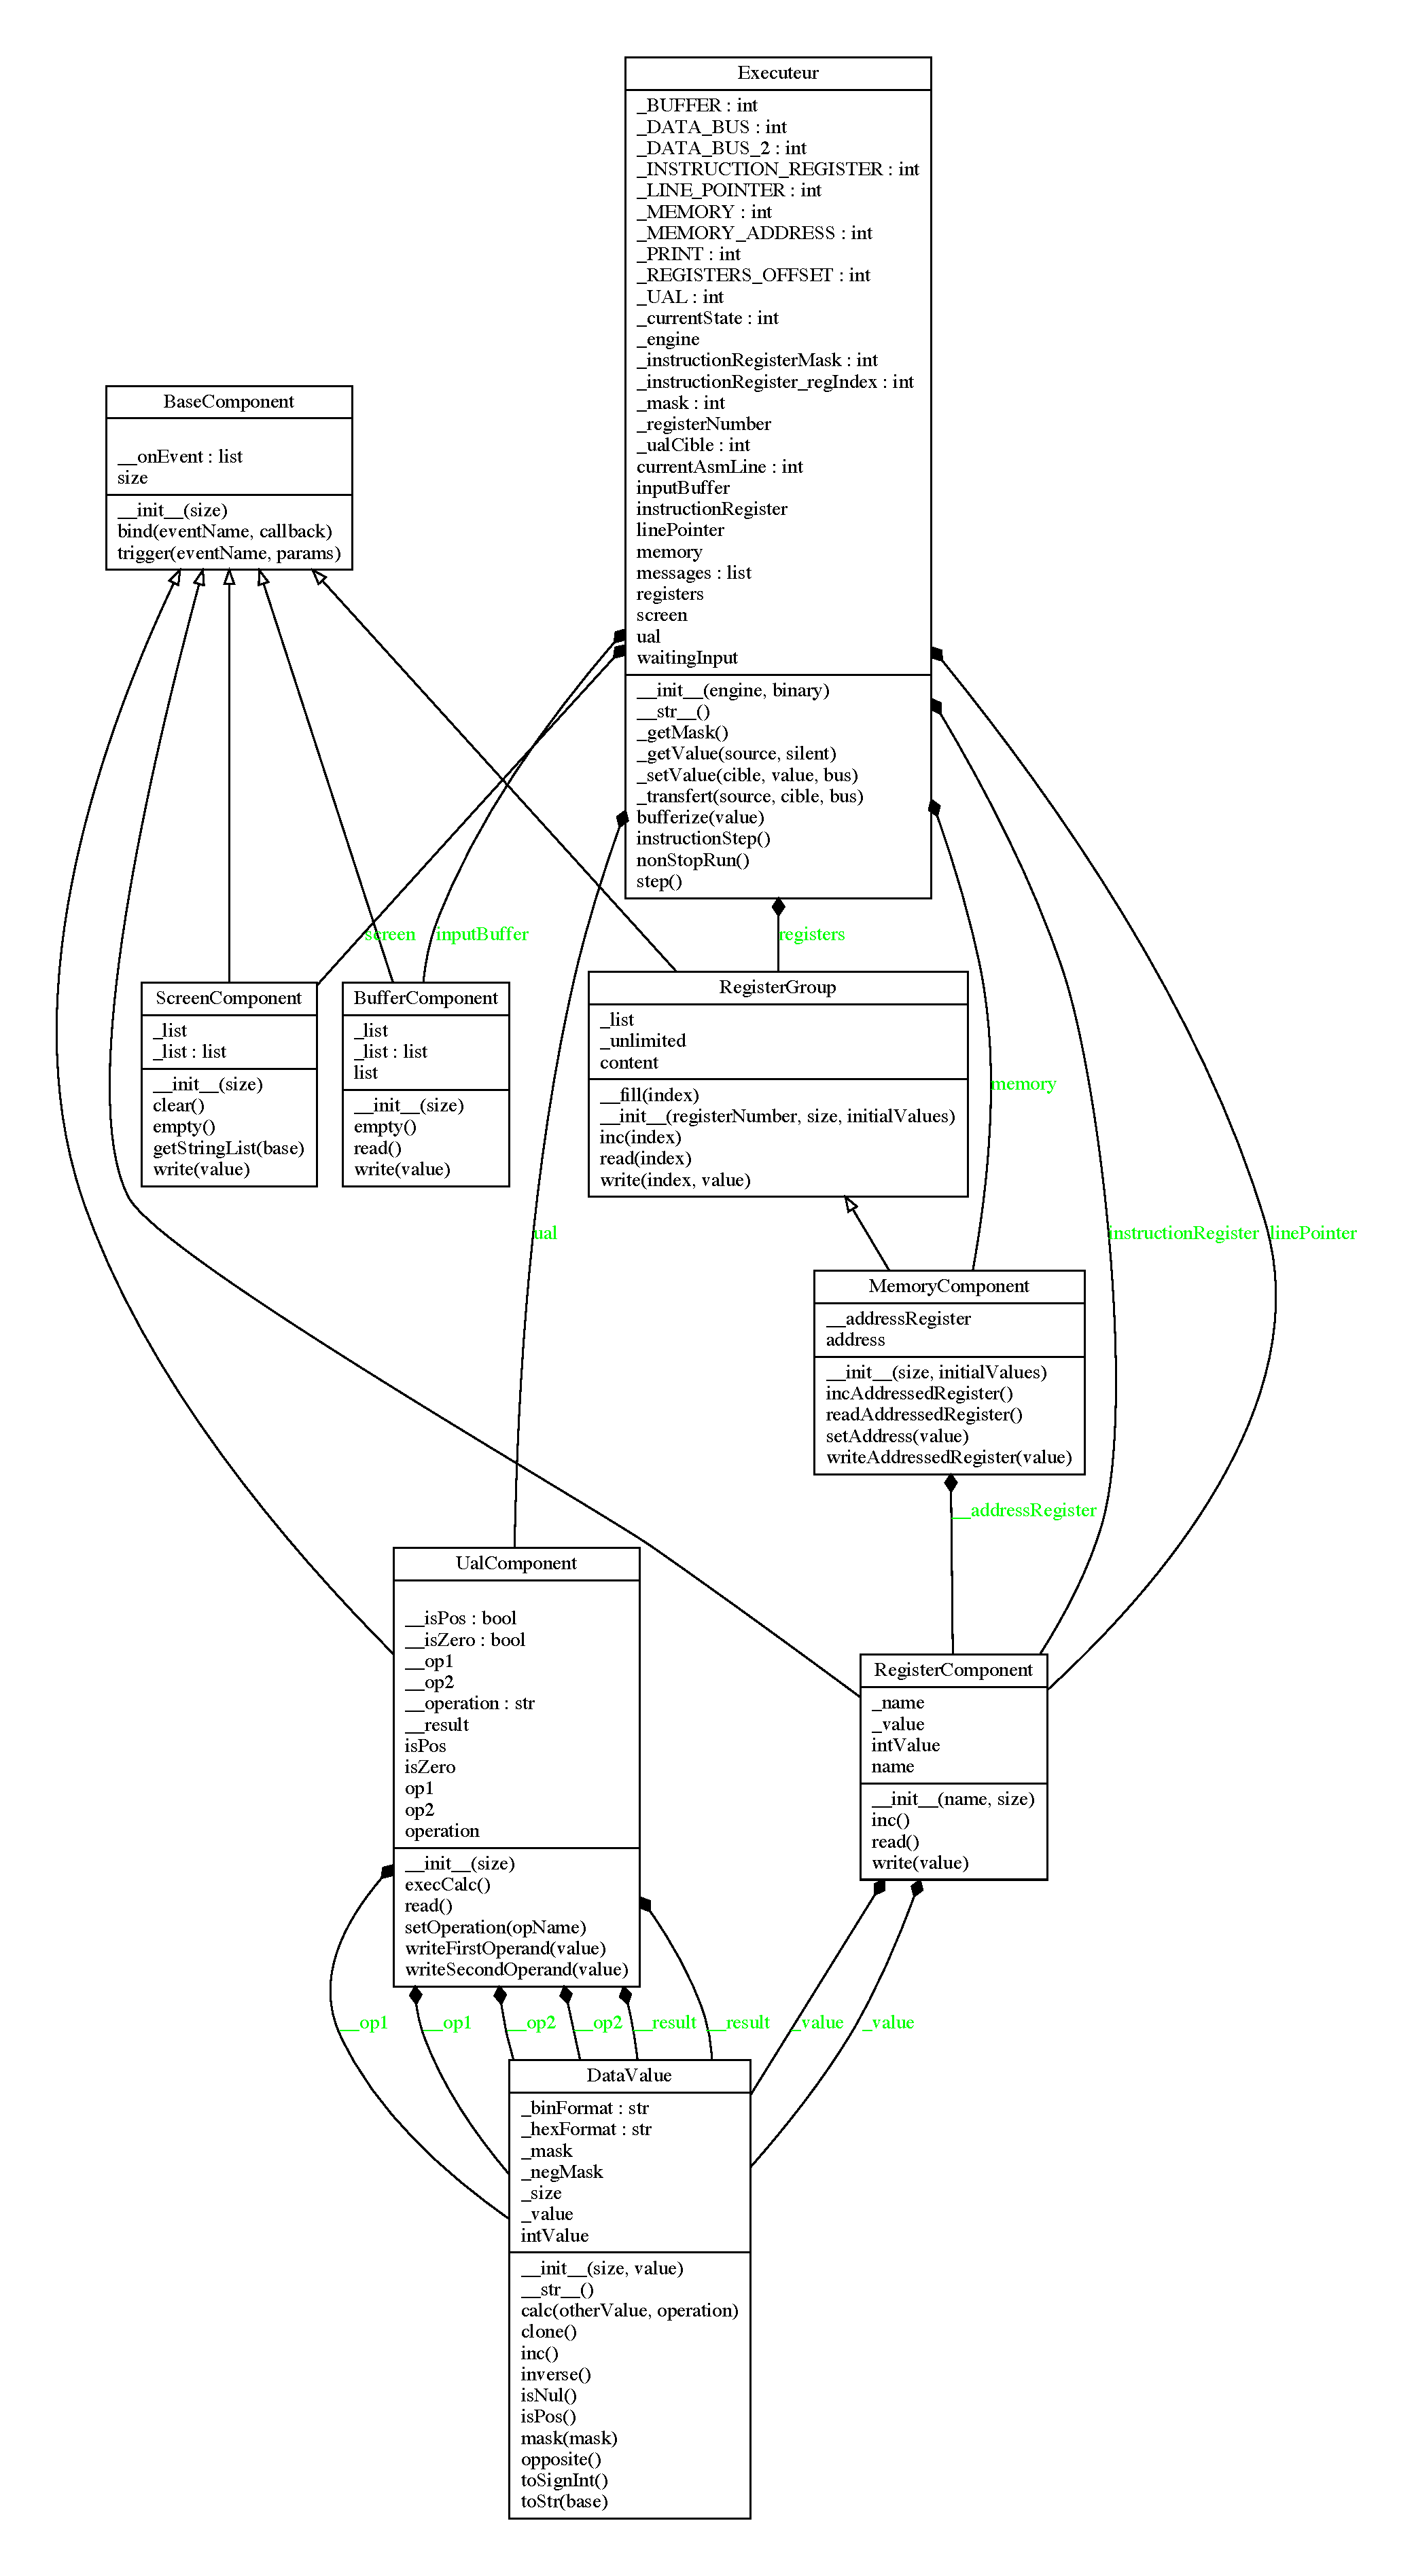
\includegraphics[height = 0.85\textheight]{./Pictures/Executeur.pdf}
	\caption{\label{fig:class_Executeur} Diagramme de classe - Executeur}
\end{figure}

\subsubsection{Executeur}

Lors de l'exécution, le processeur modèle est représenté par un objet de classe \pyinline{Executeur} (\cref{fig:class_Executeur}). Les différents paramètres (taille des registres, taille mémoire, fonctionnement UAL) sont définis par la classe \pyinline{ProcessorEngine} associée. Afin de permettre le suivi de l'exécution, l'\pyinline{Executeur} implémente entre autre:
\begin{itemize}
	\item 2 bus de données: \pyinline{_DATA_BUS} et \pyinline{_DATA_BUS_2};
	\item une mémoire: \pyinline{_MEMORY};
	\item un registre adresse mémoire \pyinline{_MEMORY_ADDRESS} et un registre instruction \pyinline{_INSTRUCTION_REGISTER};
	\item un pointeur de ligne \pyinline{_LINE_POINTER};
	\item une sortie affichage \pyinline{_PRINT};
	\item un buffer \pyinline{_BUFFER};
	\item une UAL \pyinline{_UAL}.
\end{itemize}



Chaque composant est modélisé par une instance d'une classe dédiée (\pyinline{ScreenComponent}, \pyinline{UalComponent}, \pyinline{RegisterGroup}, etc...) implémentant les méthodes associées au comportement de chaque composant physique. Par exemple pour l'UAL, (\pyinline{UalComponent}) a pour méthodes:
\begin{itemize}
	\item  \pyinline{setOperation()}: pour définir l'opération à venir;
	\item \pyinline{writeFirstOperand()}: pour mémoriser le premier opérande;
	\item \pyinline{writeSecondOperand()}: pour mémoriser le premier opérande;
	\item \pyinline{execCalc()}: pour exécuter le calcul;
	\item \pyinline{read()}: pour transférer le résultat vers le registre de sortie ;
\end{itemize}



\paragraph{Exécution}
La classe \pyinline{Executeur} a la charge de l'exécution du programme. L'exécution d'une instruction correspond à l'ensemble des étapes permettant d'évaluer un mot binaire. Chaque instruction se décompose en une série d'étapes élémentaires ou \textit{pas}. On suit l'évolution de l'exécution des différents pas à l'aide d'une variable d'état \pyinline{_currentState} (voir \cref{fig:graphe_currentState}).

Le simulateur doit permettre d'accéder aux informations processeur (usages registres, mémoires, état UAL,...) à chaque pas. Les messages à visée didactique traçant l'exécution sont stockés dans l'attribut \pyinline{messages} (voir \cref{sec:interface})

\begin{figure}
	\centering
	\tikzset{>=latex}
\begin{tikzpicture}[shorten >=1pt,node distance=3cm,on grid,auto]
\tikzstyle{command}=[sloped, align=center, font={\footnotesize\ttfamily}]

\node[state,initial,accepting] (s_0)  {$0$};

\node[state] (s_5) [above right of=s_0]  {$5$};

\node[state] (s_1) [below right of=s_5]  {$1$};

\node[state] (s_4) [above right of=s_1]  {$4$};

\node[state] (s_2) [below right of=s_4]  {$2$};

\node[state,accepting] (s_m1) [right of=s_2]  {$-1$};

\node[state] (s_3) [below of=s_1]  {$3$};

\node[state] (s_6) [above right of = s_5] {$6$};

\node[state] (s_8) [above right  = 1.5 cm and 3 cm of s_6] {$8$};
\node[state] (s_m2) [above left  = 1.5 cm and 3 cm of s_6] {$-2$};

\node[state] (s_7) [below = 1.5 cm of s_3] {$7$};

\path[->]
(s_0)	edge				node[command]				{Line pointer ->\\ reg. adresse}	(s_1)
(s_1)	edge				node[command]				{Mem. ->\\ reg. instruction}			(s_2)
(s_2)	edge				node[command]				{HALT}								(s_m1)
		edge				node[command,anchor=north]	{CMP}								(s_3)
		edge				node[command]				{Opé. (+,-,\ldots)  \\-> UAL }		(s_4)
		edge[bend left]		node[command]				{NOP, GOTO,...}						(s_0)
		edge[bend right=40]	node[command]				{STORE}								(s_6)
		edge[bend left]		node[command]				{LOAD}								(s_7)
		edge[bend right]	node[command]				{INPUT}								(s_8)
(s_3)	edge				node[command,anchor=north]	{Exécution\\UAL}					(s_0)
(s_4)	edge				node[command]				{Exécution\\UAL}					(s_5)
(s_5)	edge				node[command]				{UAL->\\reg. sortie}				(s_0)
(s_6)	edge[bend right=40]	node[command]				{reg.->mem.}						(s_0)
(s_7)	edge[bend left]		node[command]				{mem.->reg.}						(s_0)
(s_8)	edge[bend right]	node[command]				{WAIT}								(s_m2)
		edge[bend right=60]	node[command]				{Buffer->mem.}						(s_0)
(s_m2)	edge[bend right]	node[command]				{Buffer->mem.}						(s_0)
(s_m2)	edge[loop left]		node[command, anchor = south]				{WAIT}								()
;

\end{tikzpicture}
	\caption{\label{fig:graphe_currentState}Graphe exécution instruction. Etat \pyinline{currentState}}
\end{figure}


 

\clearpage